\chapter{Evaluation}

I conduct the evaluation of the project of the basis of the evaluation strategy in the project proposal.
The criteria suggested were \textbf{expressiveness}, \textbf{correctness} and \textbf{performance}, which are all reasonable to expect from a new language and compiler. 
As part of expressiveness, we consider Ein's usability as an alternative to NumPy, but also its computational limitations.
Lastly, since I introduce novel methods in this project, we discuss the \textbf{research contribution} based on external reviews received throughout the project.

\section{Expressiveness}

We evaluate the expressiveness of Ein from two perspectives: \begin{itemize}
    \item For a \textit{programmer}, what patterns are easier to express in Ein than in the established NumPy?
    \item \textit{Computationally}, what can or cannot be expressed in Ein's formal program representation, Phi?
\end{itemize}

\subsection{Programming in Ein}

I argue that Ein is a superior alternative to NumPy-like array frameworks in a variety of cases. 
Ein's design takes advantage of the pointful style and higher-order combinators. 
It introduces language features unseen in the array programming model.
On the other hand, NumPy is occasionally more concise and is much more mature as software, but often generalises badly to non-standard operations. 
To illustrate the key points, we follow a few case studies and discuss the differences between Ein and NumPy implementations.

\subsubsection{Logits in a Graph Attention Network}

Our flagship example of an unwieldy many-dimensional operation is the logit computation in a Graph Attention Network (GAT), as introduced in the very first chapter. The NumPy implementation below was paraphrased from the original real-world Jax code (the interface of which is based on NumPy):
\begin{center}
\begin{cminted}{python}
logits = (
    transpose(expand_dims(att_1, axis=-1), (0, 2, 1, 3)) +  # + [B, H, N, 1]
    transpose(expand_dims(att_2, axis=-1), (0, 2, 3, 1)) +  # + [B, H, 1, N]
    transpose(att_e, (0, 3, 1, 2)) +                        # + [B, H, N, N]
    expand_dims(expand_dims(att_g, axis=-1), axis=-1)       # + [B, H, 1, 1]
)                                                           # = [B, H, N, N]
\end{cminted}
\end{center}
We translate this into the following Ein code:
\begin{center}
\begin{cminted}{python}
def batch_logits(s, t, e, g):
    return array(lambda h, u, v: s[u, h] + t[v, h] + e[u, v, h] + g[h])
logits = array(lambda b: batch_logits(att_1[b], att_2[b], att_e[b], att_g[b]))
\end{cminted}
\end{center}
It is worth remarking that the Ein code compiles into NumPy calls which are just as efficient as the base implementation above. We move on to discuss the key differences:

\begin{description}
    \item[Shape manipulation] The array programming model revolves around manipulating the shapes of arrays to `align' them for following whole-array operations. As we discussed throughout this report, this approach does not generalise well to \textbf{many-dimensional data}. The NumPy code is polluted with \textit{axis indexing} -- and worse yet, permutations of these indices. The syntax of the operation is unhelpful in determining its actual meaning. In contrast, Ein code makes use of more mathematical, index-oriented descriptions. Extending the Ein code with another dimension simply requires the addition of another index -- rather than having to modify fragile arguments to NumPy routines. Additionally, index names serve to hint at the meaning of the respective dimensions -- like variables hint at data.
    \item[Batching] The Ein code is slightly different from what was foreshadowed in the Introduction. We separated out a \textcolor{blue}{\texttt{batch\_logits}} function, which performs most of the original's behaviour, but disregarding the \textit{batch axis}. A batch axis is a pervasive code structuring technique in NumPy code, which allows mapping the same operation over many inputs -- it is assumed it will be carried through in broadcasting, and it is present in the \texttt{att\_*} arrays. In Ein, we settle for an approach closer to functional programming, and explicitly map elements of arrays \texttt{att\_*} across each index \texttt{b}. This is clearer in intent and avoids arbitrary code conventions. Though less concise, we make data flow explicit.
\end{description}

\subsubsection{Min-plus matrix multiplication}

We now consider the case of min-plus (or \textit{tropical}) matrix multiplication, which is relevant in shortest path problems. It is defined on a pair of matrices $A$ and $B$, and the resulting matrix $D$ is given by $D_{i,k} = \min_{j} A_{i,j} B_{j,k}$ (like a usual matrix products, but in a $(\min, +)$ algebra instead of $(+, \times)$). We compare equivalently efficient NumPy and Ein implementations that compute this product in $\mathcal O(n^2)$ space.

\begin{center}    
\begin{minipage}[t]{.5\textwidth}
\raggedright
\begin{center}    
\begin{cminted}{python}
n, m = a.shape
m, k = b.shape
d = full((n, k), float("+inf"))
for t in range(m):
  d = minimum(
    d, 
    expand_dims(a[:, t], axis=1) + b[t, :]
  )
\end{cminted}
\end{center}
\end{minipage}%
\begin{minipage}[t]{.5\textwidth}
\raggedleft
\begin{center}    
  \begin{cminted}{python}


d = array(
  lambda i, j: fold(
    float("+inf"),
    lambda k, acc: min(acc, a[i, k] + b[k, j])
  )
)
  \end{cminted}
\end{center}
\end{minipage}
\end{center}

\begin{description}
    \item[Reasoning about shape] In NumPy, ndarrays possess the \texttt{shape} property. In this case, it is necessary to use this both to construct the initial accumulator array, and compute the number of loop iterations. This sort of reasoning is inconvenient. Code clarity requires introducing additional variables to the code, disconnecting their meaning as describing the structure of an array. In Ein, \textbf{size inference} takes care of assigning the right array sizes and loop iteration counts.
    \item[Data-parallel loops] To implement the matrix product in a space-efficient fashion, we need to use a matrix accumulator in NumPy. Using broadcasting to produce a cubic-size array would be more convenient, but would cause performance losses at larger problem sizes due to excessive memory use. Ein makes it simple to write data-parallel loops through its \texttt{fold} accumulator. This avoids the need to reason about the entire matrix like in NumPy, but allows focusing on the value at some index $(i, j)$.
    Arguably, Ein's \texttt{fold} syntax is far from ideal, but this could be helped here by using a short-hand like:
    \begin{center}        
    \begin{cminted}{python}
def fold_min(f):
    return fold(float("+inf"), lambda k, acc: min(acc, f(k)))
d = array(lambda i, j: fold_min(lambda k: a[i, k] + b[k, j]))
    \end{cminted}
    \end{center}
\end{description}

\subsubsection{Pairwise $L_1$ distances}

We begin with a relatively simple example which computes the sum of absolute differences ($L_1$ distance) between every pair of rows of a matrix \texttt{A}. 
% This operation has the following index-oriented specification:
% $$ \texttt{pairwiseL1(A)}_{i,j} = L_1(\texttt{A}_i, \texttt{A}_j) = \sum_k \left| \texttt{A}_{i,k} - \texttt{A}_{j,k} \right| $$
We compare NumPy (as in \cite{maclaurin2019dex}) and Ein implementations:
\begin{center}    
\begin{minipage}[t]{.5\textwidth}
\raggedright
\begin{center}    
  \begin{cminted}{python}
def pairwiseL1(A: ndarray) -> ndarray:
  return sum(
    abs(transpose(A, (1, 0)) 
        - expand_dims(A, axis=2)),
    axis=1)
  \end{cminted}
\end{center}
\end{minipage}%
\begin{minipage}[t]{.5\textwidth}
\raggedleft
\begin{center}    
  \begin{cminted}{python}
def L1(u: Vec[Float], v: Vec[Float]) -> Float:
  return reduce_sum(lambda i: abs(u[i] - v[i]))

def pairwiseL1(A: Vec[Vec[Float]]):
  return array(lambda i, j: L1(A[i], A[j]))
  \end{cminted}
\end{center}
\end{minipage}
\end{center}
\begin{description}
    \item[Separation of concerns] The Ein implementation separates the computation of $L_1$ distances into the function \textcolor{blue}{\texttt{L1}} -- this is difficult to replicate in NumPy. By forcing reasoning on whole arrays, the array programming model actively discourages encapsulation. For example, the simplest approach to extending the code to different metrics would have to be to support a fixed set -- failing the \textit{expression problem}. A higher-order function parametrised by the distance function would necessitate upholding a certain contract (e.g. the distance is computed along a certain axis). In contrast, Ein's \textcolor{blue}{\texttt{pairwiseL1}} could be rewritten to take any \texttt{dist} of the same signature as \textcolor{blue}{\texttt{L1}}:
    \begin{center}
    \begin{cminted}{python}
def pairwiseL1(A: Vec[Vec[Float]], dist: (Vec[Float], Vec[Float]) -> Float):
    return array(lambda i, j: dist(A[i], A[j]))
    \end{cminted}
    \end{center}
    Ein's rich abstractions are further discussed on the basis of our Semiring benchmark case (Section \ref{benchmarks}), where we implement abstractions that cannot be obviously replicated in NumPy.
    \item[Type signatures] NumPy's support for type signatures is poor. Type checking by standard tools like \texttt{mypy} is even more problematic, and only partially solved by bespoke extensions \cite{liu2020type}. In contrast, Ein's type system is simple and behaves well under composition. Ein code can have useful static type checking performed by \texttt{mypy}. Furthermore, \texttt{mypy} can e.g. infer the return type of \textcolor{blue}{\texttt{pairwiseL1}}, which is \texttt{Vec[Vec[Float]]}. This is a stark difference to the failings of typing NumPy programs.
\end{description}
% In addition, points we discussed prior hold just as strongly in this case -- Ein code is much clearer than the NumPy equivalent, necessitating no fragile code (e.g. from the use of axis indexing).

% \paragraph{Functions}
% \paragraph{No rank polymorphism}

\subsection{Computation in Phi}

Having considered the practicalities of Ein, we consider its computational limitations on the basis of Phi. We refer to known theory and features present in other array languages.

\paragraph{Primitive recursion} 
Phi is not Turing-complete -- all Phi programs terminate. 
We can lower bound its expressive power by primitive recursive functions (standard in computation theory). 
Indeed, our indexed \texttt{fold} directly corresponds to the primitive recursion operator $\rho$. 
Nevertheless, we argue Turing-complete computations are seldom necessary in array programming. 
Since Ein is an embedded DSL, we can rely on the generality of its host language, Python -- which is standard practice. 
% We further lack control flow primitives like conditional branches, a design choice for which we argued in the Implementation chapter -- Phi's limitations seek to meet in the middle with what is efficient in hardware.

\paragraph{Lack of in-place updates} A major computational limitation of Phi and hence Ein is the lack of support of in-place updates. 
Since Ein is purely functional, we cannot simply rely on side effects to handle updates, which leads to higher computational complexity of some algorithms. 
Efficient array implementations are problematic in functional languages in general. 
To this end, Futhark uses a uniqueness type system, while Dex makes use of an effect system \cite{henriksen2017futhark, paszke2021getting}. 

\needspace{1em}
It is worth noting in-place updates can be (unsafely) replicated through the use of extrinsics as follows: 
\begin{center}    
\begin{cminted}{python}
def update(vec: Vec[Scalar], p: Scalar, x: Scalar) -> Vec[Scalar]:
    def with_update(arr: ndarray, pos: int, val: int) -> ndarray:
        arr[..., pos] = val; return arr
    return ext(with_update, vec.expr.type)(vec, p, x)    
\end{cminted}
\end{center}
Here, \texttt{update} mutates its \texttt{vec} argument, returning \mintinline{python}{array(lambda i: where(i != p, vec[i], x))}. Careless use leads to unexpected behaviour, but the approach exemplifies how extrinsics can be used to extend Ein.


\paragraph{Parallelism} Ein offers only limited support for common computational patterns. Though associative reductions were implemented as an extension, there are many other examples of useful parallel programming patterns. These are best exemplified by Futhark's array combinators -- particularly scan, histograms (\textit{scatter} in the context of GPU programming), and filtering. I postulate these could be implemented as extensions, but only some can be efficiently interpreted by calling out to NumPy routines.

\section{Correctness}

Formally proving the correctness of compilers is difficult. 
This is owed to the gap between the practical implementation and the theoretical complexity of program analyses and transformations. 
Such an endeavour constitutes a project of its own, necessitating an implementation language that is designed for formal verification and a thorough, technical formalisation. 
I settled for a robust test suite testing runtime correctness.
% and defensive programming as a general technique to improve recall (as in detection of actual bugs). 

\subsection{Tests}

Ein's test suite (implemented in the \texttt{pytest} framework) mainly consist of compiled program output correctness in a variety of settings. 
We can distinguish three main kinds of tests of this sort:
\begin{itemize}
    \item 13 Phi/IR-level tests. These consist of small program definitions directly in the Phi calculus. They are essentially unit tests for the na\"ive Phi interpreter.
    \item 59 Ein tests of small to medium length, which are implemented through Ein's API. This includes feature-specific tests for: extrinsics (4 tests), records (7 tests), and the PyTorch backend (6 tests).
    \item 9 \textit{case} tests, which are longer. These were constructed from larger programs from various sources. We also use these for benchmarking (an overview is given in Section \ref{benchmarks}).
\end{itemize}
Most tests are parametrised by execution backend (through \texttt{pytest.mark.parametrise}) and are run repeatedly on random inputs. Since control flow in Phi is limited (e.g. all subexpressions are evaluated), random data is essentially sufficient to capture whether programs are compiled correctly. 

In some cases, output correctness cannot be checked against human-prepared values (e.g. due to problem size). Therein I instead use the na\"ive Phi interpreter, which has an implementation orthogonal to other execution backends. 
It should be noted that outputs are treated as correct even when the equality is approximate, as many tests use (inaccurate) floating point arithmetic. 
Specifics of floating point semantics are often disregarded in domains like machine learning due to the limitations they cause in optimisations -- for instance, floating point addition is not associative \cite{alawi2004every}.

The entire test suite passes successfully. The test line coverage across the implementation was measured to be \textbf{92\%}. Most of the untested code is in error paths, which were tested less often. Tests instead focus on ensuring that correct Ein/Phi programs behave correctly. Checking that bad programs fail gracefully would mostly serve to test user experience, which was not part of the success criteria.

\subsection{Defensive programming}

To improve the capability of tests to pick up bad behaviour \textit{(recall)} in internal parts of the implementation, a form of \textit{defensive programming} was applied throughout project code.
This was only a general practice of ensuring expected invariants are met through Python \mintinline{python}{assert} statements. Failing an assertion generally indicates an internal compiler error and hence a bug. We consider a few examples: \begin{itemize}
    \item Types in the array-of-structs to struct-of-arrays program transformation are mapped in a consistent way ($\phisoa{\phivectype{(\phipairtype{\tau_1}{\tau_2}})} = \phipairtype{\phivectype{\tau_1}}{\phivectype{\tau_2}}$). We assert this mapping is upheld for each subexpression.
    \item We check that outlining yields programs which are equivalent, by comparing the original program $p$ and $\mathrm{inline}(\mathrm{outline}(p))$. Therefore, we ensure let-bindings inserted preserve program semantics.
    \item We check that all Phi and Yarr terms constructed are well-typed, and that Axials meet their invariants.
\end{itemize}
By testing invariants through program assertions and including feature-specific tests, a diverse component testing suite is formed. 

\section{Performance}

Ein's code generation phase results in a Yarr program, which is by default interpreted by calling respective NumPy routines. 
Hence, our choice of compilation target (and runtime) is unique in the regard it is rather high-level.
The `machine code' is NumPy, and hence the we are limited by its performance characteristics. 
Generally it is sensible to compare compiler-generated programs against a baseline.
We form a suite of baseline NumPy programs and compare Ein's performance on a varied suite of benchmarks.

\subsection{Benchmarks}
\label{benchmarks}

We benchmark array programs generated by Ein against baseline NumPy implementations.
However, the choice of baselines is inherently subjective -- for any Ein-generated program using NumPy, there is a just as fast program using NumPy directly.
For a fair comparison, I aimed for \textit{idiomatic} NumPy code without particular optimisations applied.
We consider Ein to be efficient if at large problem sizes the running time is within a small constant factor of the baseline. 


\begin{table}
    \centering
    \begin{tabular}{c|c|l}
       \textbf{Benchmark} & \textbf{Source} & \textbf{Description} \\ \hline
        Attention & Open-source & core part of Neural Attention \\
        GAT & Open-source & inference in the Graph Attention Network architecture \\
        Semirings & Based on \textcite{dolan2013fun} & shortest paths via closure of a tropical semiring matrix \\
        MRI-Q & Parboil & basic linear reduction \\
        Stencil & Parboil & basic 3D stencil \\
        Hotspot & Rodinia & complex 2D stencil \\
        Pathfinder & Rodinia & 1D dynamic programming 
    \end{tabular}
    \caption{Brief overview of each of the Ein benchmark cases. They are also included in the test suite as system tests.}
    \label{tab:benchmarks}
\end{table}


\paragraph{Suite} Our benchmark suite builds on the findings from Section \ref{suite-review}. We mainly base on cases implemented in the Futhark benchmarks \cite{The_Futhark_Hackers_futhark-benchmarks} (particularly the Parboil and Rodinia suites, also used by Dex), as well as open-source implementations of deep learning architectures.
A comprehensive overview of these cases can be seen in Table \ref{tab:benchmarks}. I translated all of the cases from the source language (Futhark or Python using PyTorch/Jax) into equivalent a pair of programs in Python using Ein or NumPy.

A benchmark case worth special note is \textit{Semirings}. 
The NumPy baseline is a standard $\mathcal O(n^3)$ implementation of the Floyd-Warshall all-pairs shortest paths algorithm. 
In Ein, we instead apply generic record types, and make rich use of arrays of user-defined dataclass types. 
We follow the approach of \textcite{dolan2013fun} for solving a general family of problems via matrices over a \textit{closed semiring}%
\footnote{A \textit{semiring} is an algebraic structure $(+, \times)$, where the operation $+$ is a `choice' and $\times$ a `sequencing', with identity elements $0$ and $1$. \textit{Closed semirings} further define an operation $a^*$ which computes $a^* = 1 + a + a^2 + \cdots$. These structures necessarily follow certain algebraic laws. The \textit{tropical semiring} turns out to underlie the computation of shortest paths in a graph.}.
We implement their generic approach in Ein, taking advantage of efficient array operations.
% By implementing the \texttt{Tropical} instance of a \texttt{Semiring}, we can compute the closure of a generic \texttt{SemiringMatrix}, yielding the shortest paths.
NumPy lacks similarly capable abstractions, and in Ein we show they are of zero cost.
See Figure \ref{fig:semirings} for the crux of the generic Ein implementation.

\begin{figure}
    \centering
\begin{cminted}{python}
class SemiringMatrix:
    ...
    def closure(self):
        return SemiringMatrix(fold(
            self.elem,
            lambda k, acc: array2(
                lambda i, j: acc[i, j] + acc[i, k] * acc[k, k].closure() * acc[k, j]
        ).assume(self.elem[k, k]))) + self.one
\end{cminted}
    \caption{Closure of a \texttt{SemiringMatrix} in Ein (Algorithm 6.1 \cite{abdali1985transitive}). \texttt{+}, \texttt{*} are overloaded \texttt{Semiring} operations. When \texttt{+} is $\min$ and \texttt{*} is $+$, this reduces to the Floyd-Warshall shortest paths algorithm.}
    \label{fig:semirings}
\end{figure}

It is worth note that the other 2 cases used in the test suite -- NN and KMeans (from Rodinia) -- were excluded from the benchmark. A computationally efficient implementation of these relies on features unavailable in Ein (respectively in-place updates and histogram computations). They could be mimicked through extrinsics in practice, but their use would not constitute a useful benchmark.

\paragraph{Methodology} Benchmarks were conducted on a M1 Pro MacBook (14-inch, 2021). The versions used were Python \texttt{3.11.6} and NumPy \texttt{1.26.4}. No further thread parallelism was used beyond what is used by default in NumPy (in linear algebra routines). Large problem sizes are used (about 1 second of execution time), taking the minimum time across at least 5 runs. 

\begin{figure}[b]
    \centering

    \pgfplotsset{
    /pgfplots/baseline legend/.style={
    legend image code/.code={
    \draw[thick,draw,color=red](-0.05cm,0cm) -- (0.3cm,0cm);%
       }
      }
    }
    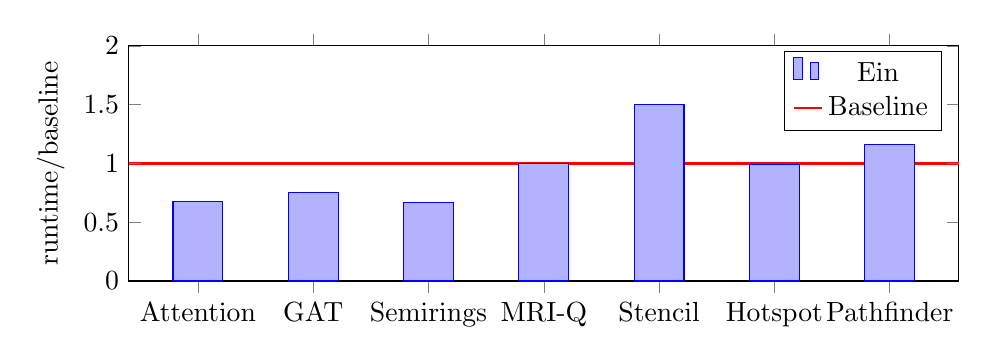
\begin{tikzpicture}
        \begin{axis}[
            ybar,
            ymin=0,
            ymax=2,
            extra y ticks = 1,
            extra y tick labels={},
            extra y tick style={grid=major,major grid style={thick,draw=red}},
            symbolic x coords={Attention, GAT, Semirings, MRI-Q, Stencil, Hotspot, Pathfinder},
            legend entries={Ein, Baseline},
            xtick=data,
            ylabel={runtime/baseline},
            bar width=1.8em,
            width=\linewidth,
            height=13em,
        ]
    
        \addplot[draw=blue, fill=blue!30] coordinates {
            (Attention, 0.68) 
            (GAT, 0.75) 
            (Semirings, 0.67)
            (MRI-Q, 1.0) 
            (Stencil, 1.5)
            (Hotspot, 0.99)
            (Pathfinder, 1.16)
        };
        \addlegendentry{Ein}
        \addlegendimage{baseline legend}
        \addlegendentry{Baseline}
    
        \legend{Ein, Baseline}
        
        \end{axis}
    \end{tikzpicture}

    \caption{Ratio of the running time of Ein-generated NumPy programs, and the baseline NumPy. \textit{Lower is better.}}
    \label{fig:benchmark-results}
\end{figure}


\paragraph{Discussion} Benchmark results can be seen in Figure \ref{fig:benchmark-results}. Results are generally promising -- Ein is no more than 60\% slower, and in some cases it is 40\% faster. 
Generally, where Ein outperforms the baseline, it is thanks to (but not limited to) operating in-place to avoid allocation of temporaries. 
Performance deficits are especially due to missing advanced indexing strategies -- particularly in Stencil. 
However, the downside of the baseline's performance is the inclusion of error-prone expressions like \mintinline{python}{A[1:-1, :-2, 1:-1]} (some 10 times).
We conclude Ein offers a good trade-off on code readability and performance.

\todothis

% \section{Usability}

% \subsection{Comparison}

% \subsection{Notation}

\needspace{5em}
\section{Research contribution}

It is difficult to objectively evaluate research contribution. 
Instead of attempting to compare it against a chosen subset of existing work, I appeal to external reviews I received on the project. 
These were from two venues -- the ACM Student Research Competition (November -- January), and a research paper submission to the ARRAY workshop at PLDI (March -- April).

\subsection{Student Research Competition}

The ACM Student Research Competition (SRC) is an opportunity for undergraduate and graduate students to present their original research and have it reviewed by judges. 
It consists of two stages -- the conference stage, with winners from each conference invited to the ACM Grand Finals. 
Prior to participation, I only had experience with a student research competition prior at the high school level.

I submitted a 3-page (plus 5-page appendix) extended abstract to the SRC at the 51st ACM SIGPLAN Symposium on Principles of Programming Languages (POPL 2024), in the undergraduate track.
It mainly concerned the core of my project with some extensions.
This work was done in late November, receiving positive reviews in December. 
I was invited to present my work at the conference in January. 
I had to prepare a poster for presentation, and slides for a brief oral presentation. 
Throughout the entire process I was supported by my supervisor, who reviewed the materials I prepared.
My work won \textbf{first prize} among undergraduates. 

As an undergraduate winner of the POPL SRC, I was invited to submit a 5-page extended abstract to the ACM SRC Grand Finals in late April. Results for this stage are due later in May.

\begin{center}
    \textcolor{blue}{TODO: Comment on submission in late April? Results likely not prior to dissertation submission. }
\end{center}

\subsection{ARRAY Workshop}

The ACM SIGPLAN International Workshop on Libraries, Languages and Compilers for Array Programming (ARRAY) concerns all aspects of array programming. 
This includes topics particularly relevant to this project: language design, embedded DSLs, paradigms, and compilation schemes.
The 10th ARRAY workshop will be colocated with the ACM SIGPLAN Conference on Programming Language Design and Implementation (PLDI) in late June 2024.

As part of the proceedings of the workshop in early April, together with my supervisor we authored a 12-page research project on the topic of this work. I wrote the main content, with my supervisor advising me on the paper structure and taking up an editorial role. 

\begin{center}
    \textcolor{blue}{TODO: Comment on results in late April.}
\end{center}


\newpage
\section{Summary}

We summarise by returning to an overview of success criteria from the proposal: \begin{description}
    \item[Embedding an array language in Python] The implemented \texttt{ein} library successfully embeds\footnote{The original proposal unfortunately contained a misunderstanding of the phrase \textit{shallow} embedding. In reality, the intended meaning was that of a \textit{deep} embedding, which would ensure access to an intermediate representation of the Phi program. This mistake was corrected after further literature search.} a pointful array language -- which we call Ein -- in Python. Ein's API builds up terms in the Phi calculus, after which it allows calling out to the compiler to evaluate the program with an execution backend. Key extensions on the proposed interface are: general \texttt{fold} and \texttt{reduce} combinators, extrinsics, rich record types, support for verifiable type annotations, and size inference.
    \item[Designing a pointful array calculus] Phi was designed successfully, and ended up building on the $\tilde F$ language due to \textcite{shaikhha2019efficient}. This further includes various extensions with respect to the proposal: fully-fledged pair types, size assertions, folds, and associative reductions.
    \item[Efficient execution backend] A novel compilation scheme was developed that allows compilation of pointful array programs (in the Phi calculus) by generating point-free array code (Yarr calculus). This directly leads to efficient execution of Ein programs by calling out to NumPy routines. The proposal left the specifics of the execution backend somewhat vague -- but we gave a thorough description of its capabilities in the Implementation chapter. A key extension was the inclusion of a PyTorch backend. It can take advantage of the existing hardware acceleration and automatic differentation implementations -- showcasing the generality of our scheme.
\end{description}
The success criteria did not elaborate on the compiler middle-end, instead focusing on the frontend and backend. The middle-end was however suitable for various extensions: the array-of-structs to struct-of-arrays transformation, outlining (common subexpression elimination and loop-invariant code motion), and size equivalence analysis.

Throughout this chapter we have seen that Ein is expressive, and can be superior in usability as an alternative to NumPy. 
It further has various language features unseen in NumPy-like frameworks.
Therefore, we have shown Phi is suitable as an abstraction for pointful array programs. 
Ein's user-facing interface is used in tests and larger programs, showcasing its practicality.
Furthermore, robust tests ensure correctness of our implementation. 
Benchmarking has shown our execution backend is efficient on a varied suite of cases. 
Ein leads to much clearer programs than what could be written by a NumPy programmer, while preserving (or even improving) performance. 
Thanks to external review, I claim that my projects is a novel research contribution.
